\documentclass[graphics]{beamer}

\usepackage{graphicx}
\usepackage{verbatim}
\usepackage{wrapfig}
\useoutertheme{shadow}
%\usecolortheme{orchid}
\usecolortheme{seahorse}


% math commands
\newcommand{\be}{\begin{eqnarray}}
\newcommand{\ee}{\end{eqnarray}}
\newcommand{\beq}{\begin{equation}}
\newcommand{\eeq}{\end{equation}}
\def\simless{\mathbin{\lower 3pt\hbox
      {$\rlap{\raise 5pt\hbox{$\char'074$}}\mathchar"7218$}}}
\def\simgreat{\mathbin{\lower 3pt\hbox
      {$\rlap{\raise 5pt\hbox{$\char'076$}}\mathchar"7218$}}} %> or of order

% variables

\def\toonscale{0.45}
\def\mboxy#1{\mbox{\small #1}}


\begin{comment}
\AtBeginSection[]{
  \frame{
    \frametitle{Outline}
    \tableofcontents[currentsection]
  }
}
\end{comment}

\title{Fast Radio Bursts
}
\subtitle{}
\author[U. Pen]{Ue-Li Pen
\\[8mm] 
}
\date{Sept 19, 2018}


\begin{document}


\begin{comment}
  \subsection{Outline}

  \frame{
    \frametitle{Outline}
    \tableofcontents
  }
\end{comment}


  \frame{
    \frametitle{CHIME}
    \begin{itemize}
      \item software telescope, fastest survey speed
      \item learn and build tools in astrophysical theory,
        computation, radio data
      \item work at sites including Algonquin (Ontario), Penticton (BC).
    \end{itemize}
%\vspace{-0.1in}
\hspace{-.4in}
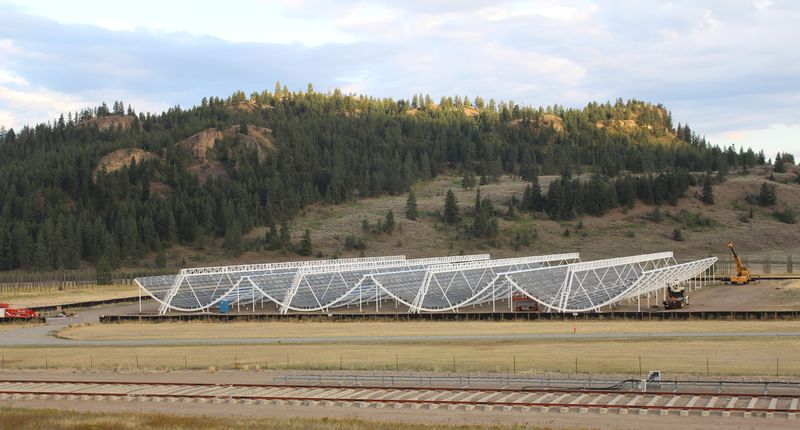
\includegraphics[width=5.05in]{Figures/800px-Full-chime-2.jpg}
}

  \frame{
\vspace{-0.5in}
    \frametitle{FRBs}
    \begin{itemize}
        \item Fast Radio Bursts: coherent sources of radio waves
        \item brightness temperatures $\sim 10^{40}$K, higher than
          Planck temperatures
        \item speculated as exploding black holes, dark matter,
          blitzars, magnetars, and more
        \item CHIME is new machine to detect and map in large numbers,
          and localize with VLBI
    \end{itemize}
\vspace{-0.2in}
\hspace{2in} 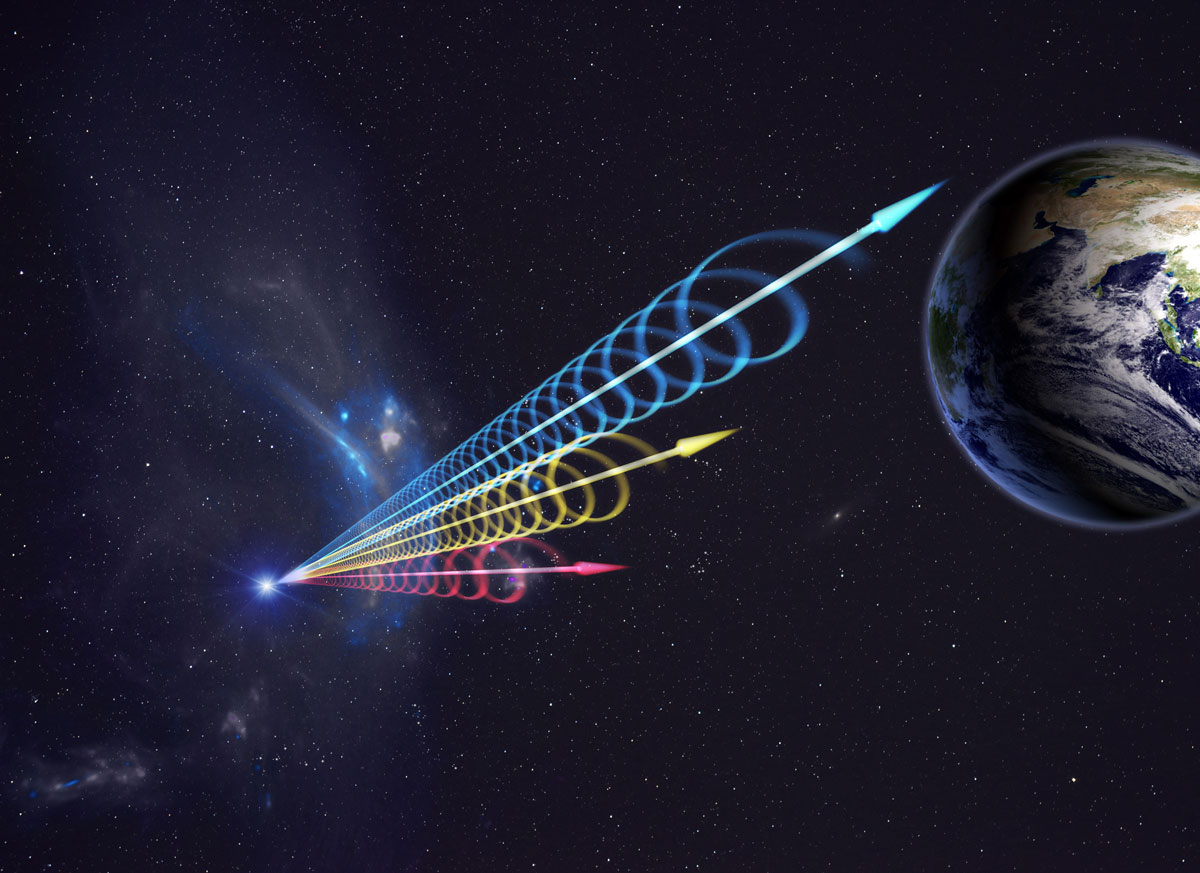
\includegraphics[width=2.05in]{Figures/FRB_nrao.jpg}
 }

\end{document}
